\documentclass[journal]{IEEEtran}
\usepackage{blindtext}
\usepackage{graphicx}
\usepackage[utf8]{inputenc}
\usepackage[brazilian]{babel}
\usepackage{lipsum}


% correct bad hyphenation here
\hyphenation{op-tical net-works semi-conduc-tor}


\begin{document}

\title{Escreva o Título do Seu Seminário Aqui}


\author{Primeiro Autor, Segundo Autor e Terceiro Autor\\

Instituto Federal de Educação, Ciência e Tecnologia da Paraíba\\Campus Campina Grande\\
E-mail:email1@mail.com; email2@mailxx.com e mail3@jjmail.com\\
}



% make the title area
\maketitle


\begin{abstract}
Escreva aqui o seu resumo. Blá blá... 
Blá blá...Blá blá...Blá blá...Blá blá...Blá blá...Blá blá...Blá blá...Blá blá...Blá blá...Blá blá...
Blá blá...Blá blá...Blá blá... Blá blá... Blá blá... Blá blá... Blá blá... Blá blá... Blá blá... Blá blá... Blá blá... 
Blá blá... Blá blá... Blá blá... Blá blá... Blá blá... Blá blá... Blá blá... Blá blá... Blá blá... Blá blá... Blá blá... 
Blá blá...Blá blá...Blá blá... Blá blá... Blá blá... Blá blá... Blá blá... Blá blá... Blá blá... Blá blá... Blá blá... 
Blá blá... Blá blá... Blá blá... Blá blá... Blá blá... Blá blá... Blá blá... Blá blá... Blá blá... Blá blá... Blá blá... 
Blá blá...Blá blá...Blá blá... Blá blá... Blá blá... Blá blá... Blá blá... Blá blá... Blá blá... Blá blá... Blá blá... 
Blá blá... Blá blá... Blá blá... Blá blá... Blá blá... Blá blá... Blá blá... Blá blá... Blá blá... Blá blá... Blá blá... 

\end{abstract}



% Note that keywords are not normally used for peerreview papers.
\begin{IEEEkeywords}
Primeira Palavra-chave, Segunda Palavra-chave, Terceira Palavra-chave.
\end{IEEEkeywords}







\section{Introdução}

Escreva aqui seu texto de introdução. 

\lipsum[3-5] % Esse comando insere texto sem sentido. Pode retira-lo daqui.


\begin{quotation}
Um exemplo de texto com citação direta. \lipsum[1-1]
Esse último comando cita uma referencia que está cadastrada no arquivo referencias.bib~\cite{mitola1999cognitive}. %Esse último comando cita uma referencia que está cadastrada no arquivo referencias.bib

%Exemplo de figura ocupando as duas colunas
\begin{figure*}[!th]
	\centering
	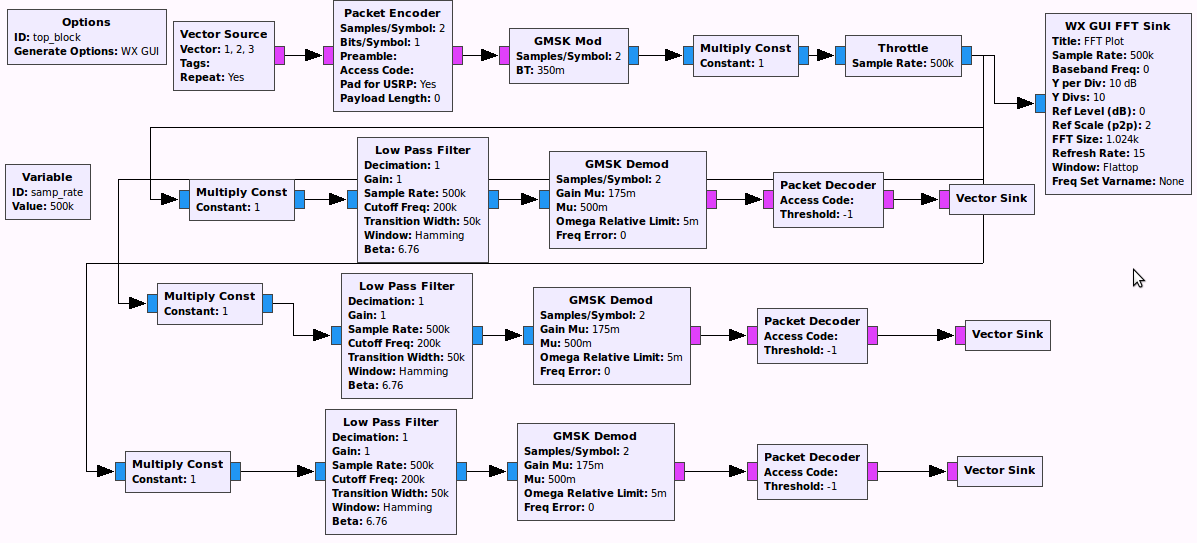
\includegraphics[width=\textwidth]{fluxo.png}
	\caption{Simulação do experimento}
\end{figure*}


\end{quotation}

\subsection{Título da Subseção}
\lipsum[1]

Veja como criar uma lista:
\begin{enumerate}
    \item Esse é o primeiro item
    \item O segundo item com uma citação~\cite{akyildiz2006next}.
\end{enumerate}


\begin{itemize}
    \item Esse é outro tipo de lista;
    \item Parece com o primeiro, mas não enumera;
    \item Pode colocar quantos quiser.
\end{itemize}


\section{Outra Seção}
\lipsum[1-2]

Figura em uma só coluna
\begin{figure}[!ht]
	\centering
	
\includegraphics[scale=0.5]{gnuradio}
	\caption{Simulação do experimento}
\end{figure}


\section{Mais uma Seção}
\lipsum[1-2]

\section{Mais uma Seção}
\lipsum[1-5]


\section{Conclusão}
Escreva aqui suas conclusões. \lipsum[1-2]

\section*{Agradecimentos}

Os autores deste trabalho agradecem ao IFPB, campus Campina Grande pelo apoio institucional. 

\bibliographystyle{IEEEtran}
\bibliography{referencias}

\end{document}


